\documentclass{hyperprior}
\title{Measuring a grader under adaptation}
\date{2026-10-18}
% Metadata are supplied by the manuscript; this specimen makes no prior claim.
\newcommand{\ExampleVersion}{specimen}
\newcommand{\ExamplePriorConfidence}{not assessed}
\newcommand{\ExampleRevisitDate}{not scheduled}
\workingpaper{\ExampleVersion}{\ExamplePriorConfidence}{\ExampleRevisitDate}
\keywords{evaluation, forecasting, code, resolution}
\begin{abstract}
A score is useful only when its interpretation survives the behaviour it rewards.
This page demonstrates the shared format used for the HyperPrior Research series.
It contains no experimental results. The layout gives the title and abstract the
full width of the page, then sets the main text in two columns. Vector figures
use the text font, a restrained palette and labels sized for the final page.
Every reported measurement in the papers is generated from a recorded experiment;
this specimen exists only to check typography and layout.
\end{abstract}
\begin{document}
\maketitle
\section{Introduction}
A grader maps a submitted forecast or program to a score. An oracle defines the
outcome against which that score is interpreted. Keeping these roles separate
makes the measurement legible: a high score can reflect correct behaviour, a
weak test, or an exposed route through the harness.

The shared format gives the two studies a common visual language. It keeps the
experimental boundary visible and leaves room for the details required to rerun
the work. Figure captions state what each display shows, then define its units
and uncertainty. They do not rely on colour alone.
\subsection{A reproducible page}
The document class controls the page dimensions, body type, section hierarchy,
header rules and caption style. It does not supply prose, results or references.
The date records the finishing day. The mark is a vector outline drawn from the
house font, so its appearance does not depend on a reader's fonts.
\begin{figure}[ht]
\centering
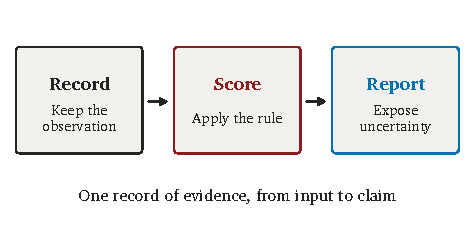
\includegraphics[width=\linewidth]{figure-example.pdf}
\caption{A shared visual system separates observations from design choices.
This diagram is a typographic specimen, with no measured values.}
\end{figure}
\section{Definitions}
For a binary outcome $y$ and a forecast $p$, the squared error is $(p-y)^2$.
The reporting code must keep its input records and record the treatment of
missing or malformed forecasts. The equations here test the mathematics font.
\begin{equation}
 S = \frac{1}{n}\sum_{i=1}^{n}(p_i-y_i)^2.
\end{equation}
The methods section specifies the sample and the scoring rule before presenting
the measurements. The results section then leads with what the study found.
\section{Method}
This specimen checks line length, paragraph spacing and the relative scale of
text and figures. It deliberately makes no empirical claim. The format review
also checks embedded fonts, PDF metadata and active links.
\subsection{Tables}
Tables align quantities by meaning and use horizontal rules sparingly. A
reproducible table is generated by the same analysis that produces its text
macros, so the two cannot silently diverge.
\begin{table}[ht]
\caption{The template assigns separate roles to each artefact.}
\centering
\begin{tabularx}{\linewidth}{lX}
\toprule
Artefact & Role \\
\midrule
Raw record & Preserve the observation \\
Analysis & Apply the declared rule \\
Figure & Show the comparison \\
\bottomrule
\end{tabularx}
\end{table}
\section{Limitations}
Page structure cannot establish the validity of a study. Its role is to expose
the evidence clearly enough that the reader can assess it. The papers retain
specific limitations alongside their measurements.
\clearpage
\section{Appendix specimen}
The later-page header carries the paper title. The footer gives the page number
and the optional working-paper metadata supplied in the preamble.
The same two-column measure is retained unless a display needs the full text
width. This page checks that the header and footer do not collide with the text.
\end{document}
